% Format teze zasnovan je na paketu memoir
% http://tug.ctan.org/macros/latex/contrib/memoir/memman.pdf ili
% http://texdoc.net/texmf-dist/doc/latex/memoir/memman.pdf
% 
% Prilikom zadavanja klase memoir, navedenim opcijama se podešava 
% veličina slova (12pt) i jednostrano štampanje (oneside).
% Ove parametre možete menjati samo ako pravite nezvanične verzije
% mastera za privatnu upotrebu (na primer, u b5 varijanti ima smisla 
% smanjiti 
\documentclass[12pt,oneside]{memoir}

% Paket koji definiše sve specifičnosti mastera Matematičkog fakulteta
\usepackage{matfmaster}
%
% Podrazumevano pismo je ćirilica.
%   Ako koristite pdflatex, a ne xetex, sav latinički tekst na srpskom jeziku
%   treba biti okružen sa \lat{...} ili \begin{latinica}...\end{latinica}.
%
% Opicija [latinica]:
%   ako želite da pišete latiniciom, dodajte opciju "latinica" tj.
%   prethodni paket uključite pomoću: \usepackage[latinica]{matfmaster}.
%   Ako koristite pdflatex, a ne xetex, sav ćirilički tekst treba biti
%   okružen sa \cir{...} ili \begin{cirilica}...\end{cirilica}.
%
% Opcija [biblatex]:
%   ako želite da koristite reference na više jezika i umesto paketa
%   bibtex da koristite BibLaTeX/Biber, dodajte opciju "biblatex" tj.
%   prethodni paket uključite pomoću: \usepackage[biblatex]{matfmaster}
%
% Opcija [b5paper]:
%   ako želite da napravite verziju teze u manjem (b5) formatu, navedite
%   opciju "b5paper", tj. prethodni paket uključite pomoću: 
%   \usepackage[b5paper]{matfmaster}. Tada ima smisla razmisliti o promeni
%   veličine slova (izmenom opcije 12pt na 11pt u \documentclass{memoir}).
%
% Naravno, opcije je moguće kombinovati.
% Npr. \usepackage[b5paper,biblatex]{matfmaster}

% Pomoćni paket koji generiše nasumičan tekst u kojem se javljaju sva slova
% azbuke (nema potrebe koristiti ovo u pravim disertacijama)
\usepackage{pangrami}

% Paket koji obezbeđuje ispravni prikaz ćiriličkih italik slova kada
% se koristi pdflatex. Zakomentarisati ako na sistemu koji koristite ovaj
% paket nije dostupan ili ako ne radi ispravno.
%\usepackage{cmsrb}

% Ostali paketi koji se koriste u dokumentu
\usepackage{listings} % listing programskog koda

% Datoteka sa literaturom u BibTex tj. BibLaTeX/Biber formatu
\bib{matfmaster-primer}

% Ime kandidata na srpskom jeziku (u odabranom pismu)
\autor{Филип Лазић}
% Naslov teze na srpskom jeziku (u odabranom pismu)
\naslov{Оптимизација целовитог програма на компајлерској инфраструктури LLVM}
% Godina u kojoj je teza predana komisiji
\godina{2021}
% Ime i afilijacija mentora (u odabranom pismu)
\mentor{др Иван \textsc{Чукић}, редован професор\\ Универзитет у Београду, Математички факултет}
% Ime i afilijacija prvog člana komisije (u odabranom pismu)
\komisijaA{др Милена \textsc{Вујошевић}, ванредни професор\\ Универзитет у Београду, Математички факултет}
% Ime i afilijacija drugog člana komisije (u odabranom pismu)
\komisijaB{др Саша \textsc{Малков}, доцент\\ Универзитет у Београду, Математички факултет}
% Ime i afilijacija trećeg člana komisije (opciono)
% \komisijaC{}
% Ime i afilijacija četvrtog člana komisije (opciono)
% \komisijaD{}
% Datum odbrane (obrisati ili iskomentarisati narednu liniju ako datum odbrane nije poznat)
\datumodbrane{15. јануар 2016.}

% Apstrakt na srpskom jeziku (u odabranom pismu)
\apstr{%
}

% Ključne reči na srpskom jeziku (u odabranom pismu)
%\kljucnereci{анализа, геометрија, алгебра, логика, рачунарство, астрономија}

\begin{document}
% ==============================================================================
% Uvodni deo teze
\frontmatter
% ==============================================================================
% Naslovna strana
\naslovna
% Strana sa podacima o mentoru i članovima komisije
\komisija
% Strana sa posvetom (u odabranom pismu)
\posveta{Мами, тати и деди}
% Strana sa podacima o disertaciji na srpskom jeziku
%\apstrakt
% Sadržaj teze
\tableofcontents*

% ==============================================================================
% Glavni deo teze
\mainmatter
% ==============================================================================

% ------------------------------------------------------------------------------
\chapter{Увод}
% ------------------------------------------------------------------------------
% ------------------------------------------------------------------------------
\chapter{LLVM компајлерска инфраструктура}
\label{chp:LLVM}
% ------------------------------------------------------------------------------

LLVM({\lat Low Level Virtual Machine}[1]), упркос свом имену LLVM мало тога има са
виртуелним машинама, то је колекција алата(компајлера, асемблера, дибагера, линкера)
који су дизајнирани да буду компатибилни са постојећим алатима пре свега на 
Unix системима.
Ови алати  се могу користити за развој front-end-a за било који програмски језик, 
као и за развој back-end-a за сваку компјутерску архитектуру.
LLVM је започет као истраживачки пројекат на Универзитету Илиноис са циљем да 
пружи статичку и динамичку компилацију програмских језика. 
Данас, LLVM садржи велики број подпројеката који се користе у великом обиму 
што у продукцијске што у истраживачке сврхе.
\newline Неки од најбитнијих подпројеката су:
\begin{enumerate}
\item Језгро LLVM-a које садржи све потребне алате и библиотеке за конверзију
међурепрезентације у објектне фајлове 
\item Clang - front-end за  C, C++ и Objective C програмске језике
\item libc++ - имплементација C++ стандардне библиотеке
\item LLDB - дибагер
\item LLD - линкер
\end{enumerate}

\section{LLVM међурепрезентација}
LLVM међурепрезентација (LLVM IR[2]) базирана je на статичкој 
јединственој форми доделе(SSA[3]).
Ова форма захтева да се свакој променљивој вредност додели тачно једном, као и да
свака променљива буде дефинисана пре употребе.
LLVM међурепрезентација је дизајнирана тако да подржи интерпроцедуралне оптимизације,
анализу целог програма, агресивно реструктуирање програма итд.
Веома битан аспект LLVM међурепрезентацијe је то што је она дефинисана као 
језик са јасно дефинисаном семантиком.
Ова међурепрезентација се може користити у три различите форме: 
\begin{enumerate}
\item текстуални асемблерски формат(.ll)
\item биткод  формат (.bc)
\item унутар-меморијски формат 
\end{enumerate} 
Овим се омогућавају ефикасне компајлерске транформације и анализе, уз могућност
визуалне анализе и дебаговања трансформација. 
Сва три формата су еквивалентна и лако се могу трансформисати један у други без
губитка информација. 
У овом раду највише ћемо се фокусирати на текстуални формат и под међурепрезентацијом
подразумевано ћемо мислити на овај формат, који се може окарактерисати као асемблерски 
језик независтан од специфичне платформе.

Овде видимо две функције у програмском језику С које сабирају 2 броја.
\begin{lstlisting}
unsigned add1(unsigned a, unsigned b) {
  return a+b;
}
// Rekurzivna funkcija za sabiranje 2 broja.
unsigned add2(unsigned a, unsigned b) {
  if (a == 0) return b;
  return add2(a-1, b+1);
}
\end{lstlisting}

Сада ћемо представити одговајући к\^{o}д у LLVM међурепрезентацији.
\begin{lstlisting}
define i32 @add1(i32 %a, i32 %b) {
entry:
  %tmp1 = add i32 %a, %b
  ret i32 %tmp1
}

define i32 @add2(i32 %a, i32 %b) {
entry:
  %tmp1 = icmp eq i32 %a, 0
  br i1 %tmp1, label %done, label %recurse

recurse:
  %tmp2 = sub i32 %a, 1
  %tmp3 = add i32 %b, 1
  %tmp4 = call i32 @add2(i32 %tmp2, i32 %tmp3)
  ret i32 %tmp4

done:
  ret i32 %b
}
\end{lstlisting}

LLVM међурепрезентација је асемблерски формат сличан апстрактном RISC[4] скупу
инструкција, са додатним структурама вишег нивоа.

Као што видимо у овом примеру, међурепрезентација подржава линеарне секвенце
једноставних инструкција као што су сабирање, одузимање, гранање, упоређивање итд.
Све ове инструкције су у тро-адресној форми, што значи да могу примити два регистра 
као улаз и резултат уписати у трећем регистру.
Међурепрезентација је строго типизирана (на пример i32 означава тридесетдвобитни
целобројни број), док се позив функције означава кључном речи call, а повратна
вредност са ret.
LLVM не користи фиксан број регистара, већ има бесконачан број променљивих које
почињу карактером \%. 
Функције и глобалне променљиве пре свог назива садрже карактер @.
Унутар репрезентације постоје и лабеле, тело сваке функције почиње лабелом begin.

\section{LLVM компајлер}  

Процес компилације у LLVM инфраструктури започиње у front-end делу који производи
међурепрезентацију, која се затим шаље алату за оптимизацију који трансформише
к\^{o}д кроз велики број оптимизација.
Потом се трансформисани к\^{o}д преводи у асемблерски к\^{o}д на жељеној архитектури, 
и на крају се асемблерски к\^{o}д преводи у машински. 
Овај процес, наравно поједностављен, можемо видети на слици испод. 

\begin{figure}[!ht]
  \centering
  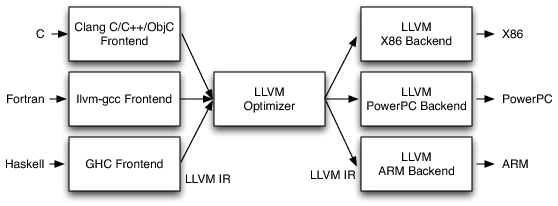
\includegraphics[width=0.8\textwidth]{LLVMCompiler1.png}
  \caption{LLVM процес компилације}
  \label{fig:grafikon}
\end{figure}

\subsection{Frond-end}
 Frond-end је задужен за парсирање, валидацију и проналазак грешака у изворном
 к\^{o}ду, затим за превођење парсираног к\^{o}да у LLVM међурепрезентацију.
 Превођење се обично извршава, прво изградњом AST-а[5], а затим 
 и превођењем AST-а у међурепрезентацију.
 У суштини сваки програмски језик, уколико имплементира front-end који може да
 изгенерише LLVM међурепрезентацију, може користити алат за оптимизацију или 
 back-end део LLVM-а.
 Постоји више пројеката који имплементирају LLVM front-end, али најбитнији су:
 
 \begin{enumerate}
 \item Clang - front-end за  C, C++ и Objective C програмске језике
 \item DragonEgg - GCC плагин који користи LLVM архитектуру за оптимизацију и 
 				 и генерисање машинског кода
 \end{enumerate}

 \subsection{Алат за оптимизацију}
 Алат за оптимизацију (eng. optimizer[6]) дизајниран је тако да на улазу прима LLVM
 међурепрезентацију, изврши оптимизације над међурепрезентацијом и после тога генерише
 измењену међурепрезентацију, која би требало да се извршава брже.
 Овај алат је организован у више низова оптимизациних пролаза, тако да је излаз
 једне оптимизације улаз у другу.
 Неки од примера оптимизационих пролаза су инлајновање, елиминација мртвог кода,
 реалокација израза, инваријација петљи итд. 
 Од нивоа оптимизације зависе и оптимизациони пролази који ће бити покренути,
 на пример, у случају Clang-a, на нивоу -O0 нема оптимизација, док на нивоу
 -O3 покреће се свих 67 оптимизационих пролаза.
 Алат за оптимизацију се може покренути командом opt.

\subsection{Back-end} 
LLVM back-end је фаза у којој се од међурепрезентације, која је улаз за ову фазу,
генерише машински к\^{o}д за специфичну архитектуру.
Главна компонента back-end-а је генератор к\^{o}да (eng. LLVM code generator[7]) који
користи сличан приступ као алат за оптимизацију, то јест дели генерисање машинског
к\^{o}дa на мање пролазе, који имају за циљ генерисање најбољег могућег к\^{o}да.
Неки најбитнији пролази су бирање инструкција, алокација регистара, распоређивање
(eng. scheduling).
LLVM може генерисати код за велики број архитектура, неки од њих су: x86, ARM,
PowerPC, SPARC.

\section{Предности LLVM-a}

LLVM пројекат је бесплатан и његов изворни к\^{o}д је у потпуности доступан, 
што је навело не само истраживаче са универзитета, већ и велики број компанија 
да учествују у његовом развоју, тако да данас значајан број људи активно 
учествује у одржавању и унапређивању овог пројекта.
Модуларни дизајн омогућава лако мењање постојећих алата или додавање нових.
Захваљујући овом дизајну врло лако је додати нови front-end, back-end или
оптимизациони пролаз.
Такође, LLVM подржава и:
\begin{enumerate}
\item JIT компилацију[8]
\item Clang-ов алат за статичку анализу к\^{o}да (eng. static code analyzer[9]) 
- који служи за  проналазак могућих грешака у коду
\item оптимизацију током линковања(LTO[10])
\end{enumerate}
 Очекује се да LLVM у потпуности замени GCC у блиској будућности.

\chapter{Оптимизација целовитог програма}

Обично изворни к\^{o}д програма делимо у више посебних фајлова(eng. source code).
Компајлер чита фајл по фајл и за сваки генерише њему одговарајући објектни фајл,
то јест сваком фајлу одговара један објектни фајл.
Овако чинимо наш к\^{o}д читљивијим, омогућавамо паралелелно компајлирање више 
фајлова али и избегавамо потребу за компајлирањем целог програма за сваку промену
у узворном к\^{o}ду.
Овакав приступ има и лошу страну, пошто компајлер преводи фајл по фајл, он нема 
информације о к\^{o}ду који се налази у другим објектним фајловима.
Због тога је немогуће извршити многе оптимизације, због тога што компајлер не може 
бити сигуран у семантичку еквивалентност.
Овај проблем се може решити уз помоћ линкера, приступом познатијим као 
оптимизација током линковања(LTO) или спајањем свих фајлова у један и извршавањем
оптимизација на једном великом фајлу.
\\
Сада ћемо на једном малом примену показати због чека оптимизација целовитог програма 
може бити корисна.

\begin{lstlisting}
//a.h                             //a.cpp
void do_nothing();                void do_nothing(){} 

//main.cpp          
#include "a.hpp"

int main(){
    for (int i = 0; i < 1'000'000'000; i++){
        do_nothing();
    }
}
\end{lstlisting}

Видимо у примеру да функција  do{\_}nothing, као и што јој име каже, не ради ништа.
Уколико овај к\^{o}д преведемо са -О3 оптимизацијом, без оптимизације целовитог програма,
добићемо овај резултат.

\begin{lstlisting}
clang++  main.cpp a.cpp  -O3
time ./a.out 
real    0m1,022s
user    0m1,014s
sys     0m0,000s
\end{lstlisting}
Видимо да је рачунару било потребно више од једне секунде са програм који не ради ништа.
Сада ћемо исте фајлове превести са оптимизацијом целовитог програма.
\begin{lstlisting}
clang++  main.cpp a.cpp  -O3 -flto=full
time ./a.out 
real    0m0,003s
user    0m0,003s
sys     0m0,000s
\end{lstlisting}

Разлика је у времену извршавања је очигледна.
Једноставно без активне оптимизације целовитог програма, алат за оптимизацију није могао бити
сигуран шта функција do{\_}nothing заправо ради, и програм је позивао исту милион пута у петљи,
док је са активном оптимизацијом могао да види к\^{o}д функције и да  оптимизује петљу.

//TODO dodaj LLVM IR

\section{Ортимизација током линковања}


Захваљујући модуларном дизајну LLVM-a и чињеници да можемо компајлирати део к\^{o}да,
сачувати резултати и наставити компилацију касније без губитака информација
слику 2.1 можемо проширити са линкером и оптимизацијама током овог процеса.

\begin{figure}[!ht]
  \centering
  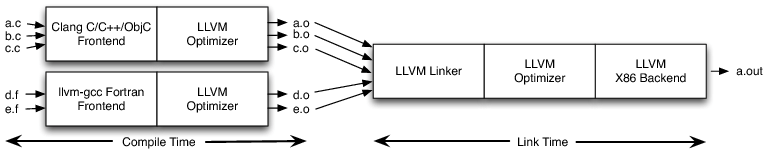
\includegraphics[width=0.8\textwidth]{LTO.png}
  \caption{LLVM процес компилације са подршком линкера}
  \label{fig:grafikon}
\end{figure}


У наставку ћемо објаснити због чека је линкер користан у оптимизацији целовитог програма.

Главни задатак линкера је да све објектне фајлове споји у један фајл, извршни фајл
или дељену библиотеку. 
Да би испунио овај задатак линкер прво мора да извши реалокацију симбола и резолуцију
симбола.
Симболи могу бити глобалне променљиве, функције, класе итд. 
Сваки објектни фајл садржи табелу симбола у којој се налазе сви симболи који 
могу бити дефинисани у истом објектном фајлу или у неком другом.
Уколико симбол није дефинисан унутар објектног фајла он ће у табели симбола бити
означен као "extern", у супротном биће означен као "import".
Да би се успешно превео програм у извршни фајл, линкер мора да пронађе све 
недостајуће симболе у свим објектним фајловима и да упише њихове адресе (такође задатак
линкера је да и неким импортованим симбола промени адресу, уколико је компајлер то назначио),
то јесте да изврши резолуцију и реалокацију симбола.
Због ових својстава линкер има круцијалну улогу у оптимизацији целовитог програма, јер
има увид у све табеле симбола и алат за оптимизацију може то искористити за оптимизације
делова к\^{o}да који су му пре били "невидљиви". 
\\
У наставку приказаћемо интеракцију између линкера и алата за оптимизацију.
Оптимизација током линковања у LLVM инфраструктури садржи четири фазе:
\begin{enumerate}
\item Читање битк\^{o}д фајлова
\item Резолуција симбола
\item Оптимизовање биткод фајлова
\item Резолуција симбола након оптимизације
\end{enumerate}

\subsection{Читање битк\^{o}д фајлова}
Сви објектни фајлови долазе до линкера, који из њих чита и сакупља информације
о симболима, који су присутни у фајловима.
Ови фајлови могу бити у форми LLVM битк\^{o}д фајлова или стандардних објектних
фајлова (eng. native object files).
Линкер већ има могућност за третирање објектних фајлова, да би могао
правилно да чита и LLVM битк\^{o}д фајлове потребна му је помоћ, а то му омугућава
алат под називом libLTO[11].
libLTO је библиотека који је намењена за коришћење од стране линкера.
libLTO пружа стабилан интерфејс, тако да је могуће користити
LLVM алат за оптимизацију, без потребе за излагањем интерног LLVM к\^{o}да.
Такође, још једна предност овог алата је то што можемо мењати LLVM LTO к\^{o}д независно
од линкера, то јесте не морамо за сваку промену к\^{o}да мењати и линкер.
\\
Да се вратимо на фазу читања битк\^{o}д фајлова, уколико линкер добије
објектни фајл, он већ зна да чита тај фајл и додаће симболе у глобалну табелу симбола.
Уколико је у питању LLVM битк\^{o}д фајл, линкер ће позвати функције \\
lto{\_}module{\_}get{\_}symbol{\_}name и 
lto{\_}module{\_}get{\_}symbol{\_}attribute 
libLTO алата да би добио све дефинисане  симболе, затим ће те симболе, 
као у случају стандардног објектног фајла, додати у глобалну табелу симбола.

\subsection{Резолуција симбола}
Као што је већ објашњено изнад, линкер покушава да разреши све симболе помоћу
глобалне табеле симбола.
Уколико је укључена опција елиминације мртвог кода, која је подразумевано укључена
уколико се користи оптимизација током линковања, линкер чува листу симбола који
су коришћени у осталим објектним фајловима, такозвани живи симболи.

\subsection{Оптимизација битк\^{o}д фајлова} 
У овој фази линкер користи информације из глобалне табеле симбола, и пријављује
живе симболе алату за оптимизацију
lto{\_}codegen{\_}add{\_}must{\_}preserve{\_}symbol функцијом.
Затим линкер позива алат за отимизацију и генератор к\^{o}да над битк\^{o}д фајловима
функцијом lto{\_}codegen{\_}compile чији је резулат објектни фајл
који настао спајањем више битк\^{o}д фајлова, са примењеним оптимизацијама на њима.
Примећујемо да је оптимизације могуће извршити искључиво на битк\^{o}д фајловима,
то јест објектни фајлови се не оптимизују.

\subsection{Резолуција симбола након оптимизације}
Сада линкер чита оптимизоване објектне фајлове и ажурира табелу симбола уколико 
има неких промена. На примера уколико је укључена елиминација мртвог к\^{o}да,
линкер може да избаци неке симболе из табеле.
У овој фази сви фајлови су објектни фајлови и линковање се наставља
по старом принципу, као да никада нису ни постојали битк\^{o}д фајлови.

\section{Отпимизација целовитог програма без подршке линкера}
Приступ отимизације целовитог програма са линкером захтева Gold[12] линкер,
који у себи има подршку за libLTO библиотеку.
На неким системима овај линкер није доступан и ту је немогуће извршити стандардну
оптимизацију током линковања.
Алтернативни приступ је спајање свих LLVM битк\^{o}д фајлова у један битк\^{o}д фајл
и извршавање оптимизација над тим фајлом.
Ово је могуће захваљујући LLVM алату llvm-link[13].
\\
Са овим приступом добијамо исте перфомансе као са приступом где имамо подршку линкера,
са тим што овај приступ неће радити уколико сви фајлови нису  битк\^{o}д фајлови,
односно не ради са објектним фајловима.

//TODO nacrtaj grafik

\section{Инлајновање функција}

Неписано правило у програмирању је издвајање к\^{o}да који се понавља у 
засебне функције.
Издвајање к\^{o}да је корисно зато што на тај начин избацујемо копирање
истог к\^{o}да на више места у програму.
На тај начин не само да повећавамо читљивост програма, већ и смањујемо
могућност грешака, које су честе при копирању  к\^{o}да.
Са друге стране, позиви функција могу бити захтевни што се тиче времена извршања.
Када се функција позове долази до креирања новог стек фрејма, померања показивача
инструкција на почетак те функције, чувања тренутног стања позиваоца функције у 
регистрима и слично.
Такође,  к\^{o}д функције може бити ван кеша инструкција, што може битно
утицати на време извршавања програма.
Решење ових проблема је инлајновање функција(eng. function inlining[14]), простим
речима инлајновање је уметање целовитог к\^{o}да функције уместо позива функције.
Ово изгледа као добра предност инлајновања, али још већа предност је то што 
сада компајлер може да генерише оптималнији  к\^{o}д.
Пошто је цео к\^{o}д функције уметнут, компајлер може извршити оптимизације у већем
блоку, што некада може довести до значајних убрзања.
Видели смо да инлајновање функција може бити корисно и намеће се логично питање-
када можемо извршити инлајновање?
Неке функције можемо одмах елиминисати, уколико имамо дељену библиотеку ми немамо
информацију о к\^{o}ду функције тако да је не можемо инлајновати.
Сличан проблем је са функцијама које се налазе у другим објектним фајловима, али за
овај проблем постоји решење, а то је оптимизација целовитог програма.
Уколико је оптимизација целовитог програма укључена, компајлер може видети
к\^{o}д функција из других објектних фајлова и евенутално их инлајновати.
Такође, немогуће је инлајновати функције које садрже инструкције индиректног
гранања(eng. indirect branch instructions[15]) јер у том случају, уколико би 
инлајновали функцију, индиректне гране би нас довеле до неочекиваних инструкција
у програму.
Видели смо неке од ситуација у којима је немогуће инлајновати функцију, као и да
инлајновање има велики број предности, да ли онда увек инлајновати када је то 
могуће?
Наравно, одговор је не. 
Поред великог броја предности, инлајновање има и неке мане.
Једна од мана је повећање величине извршног фајла, поготово када функције имају
велики број инструкција.
Видимо да ипак мора да постоји компромис између перфоманси програма и величине
извршног фајла.
Такође, функције са великим бројем инструкције могу да утичу на перфомансе, тако
што утичу на кеш инструкција, јер велики број инструкција руши локалност референци.
Због свега наведеног за инлајновање користимо хеуристике, преко којих одређујемо
да ли неку функцију треба инлајновати или не.
Битне информације које користе хеуристике су колико функција има инструкција,
колико пута се позива у току програма, да ли је функција коришћена у осталим
објектним фајловима и слично.
Поред ове статичке анализе функција, где користимо фиксиране границе(eng. threshold)
за број иснтрукција, позива итд. и тако одређујемо да ли треба да инлајнујемо функцију,
постоји и динамчка анализа.
Динамичка анализа користи информације које се добијају приликом профајлирања програма.
На овај начин можемо добити прецизније информације и самим тим боље перфомансе,
али само у случају да тестно окружење програма симулира реалну ситуацију у којој
ће се програм извршавати.
У супротном можемо добити лошије перфомансе него статичком анализом.
Профајлирањем можемо открити делове к\^{o}да који се чешће извршавају, и компајлер 
поклања посебну пажњу оптимизовању и инлајновању тих делова, јер уколико се неке
функције скоро никада не позивају, инлајновањем нећемо добити никакве предности
у перфомансама, само можемо повећати величину извршног фајла.
Уколико смо сигурни да ће неки део к\^{o}да да се често извршава, то можемо назначити
компајлеру(у C++ програмском језику) атрибутом [[likely]], без потребе за
профајлирањем. 	
Програмер може у извнорном коду сигнализирати компајлеру да изврши инлајновање
атрибутом always{\_}inline, на системима Unix, али ни то не гарантује да ће на крају
функција заиста бити инлајнована.
//TODO primeri bencmarci


\section{Елиминација мртвог к\^{o}да}

Елиминација мртвог к\^{o}да(eng. dead code elimination[16]) је компајлерска 
оптимизација која елиминише к\^{o}д који не утиче на резултат извршавања
програма.
Уклањања мртвог к\^{o}да има многе предности: смањује величину извршног програма,
побољшава локалност инструкција, уклањањем непотребних инструкција такође
повећава брзину извршавања програма.
Без укључене оптимизације целовитог програма компајлер може да елинише локалне
променљиве, инлајноване статичке функције као и статичке глобалне променљиве.
То ради једноставним праћењем позива свих статичких глобала и сврставањем истих
у живе или мртве скупове, у зависности да ли се глобал користи или не.
Све глобале из мртвог скупа, на крају оптимизационих пролаза, можемо елиминисати.

//TODO primer 

Са укљученом оптимизацијом целовитог програма можемо избацити не само статичке
глобалне променљиве или функције, него све глобале који се не користе.
Овај поступак се извршава током линковања и описан је у секцији  3.1.

/TODO primer

\section{Девиртуализација}
 Девиртуализација(eng. devirtualization[17]) је поступак замене виртуелних позива
 функција директним позивима.
 Виртуелни позиви функција су неколико пута спорији од директних, што у системима
 где се перфомансе јако вреднују може да буде велики проблем, због тога је понекад
 неопходно извршити девиртуелизацију.
 Девиртуализација се најефикасније може извршити уз помоћ оптимизације целовитог
 програма, али постоје и случајеви у којима је могуће извршити девиртуализацију 
 и без оптимизације целовитог програма.
 За почетак ћемо се позабавити тим случајевима.
 
 \subsection{Познат динамички тип објекта}
 Уколико нам је познат динамички тип објекта при компајлирању, компајлер може 
 да девиртуализује позив функције.
 
 \begin{lstlisting}
struct Base{
    virtual int f(){return 1;}
};

struct Derived : public Base{
    int f() override {return 2;}
};

int main(){
    Derived d;
    Base * b = new Base();
    b->f();
    d.f();  
}
 Primer 3.5.1
 \end{lstlisting}

 //todo llvm primer
 
 Као што видимо у примеру изнад, компајлер успешно девиртуализује ове функције
 јер зна при компајлирању да променљива b садржи објекат типа Base, док променљива
 d садржи објекат типа Derived.
 Наравно увек када променљива садржи објекат неког типа, а не показивач или референцу,
 компајлер ће моћи да девиртуализује тај позив(као у примеру променљиве d)
 
 \subsection{Кључна реч final}
 
 Искористићемо пример сличан примеру 3.5.1
 
\begin{lstlisting}
struct Base{
    virtual int f(){return 1;}
};

struct Derived : public Base{
    int f() override {return 2;}
};
int func(Derived *d){
    return d->f();
}

Primer 3.5.2
\end{lstlisting}
 
 За разлику од примера 3.5.1 овде смо структуру Derived обележили кључном 
 речју final.
 То говори комапјлеру да ни у овој, али ни у било којој другој јединици превођења, 
 не може постојати структура која је изведена из структуре Derived.
 То сазнање омогућава компајлеру да изврши девиртуализацију позива функције f().
 Примећујемо када не би експлицитно обележили  Derived са final девиртуализација
 не би била могућа, јер компајлер не може да зна да ли у некој другој јединици превођења
 постоји структура изведена из структуре Derived и самим тим преправљена фунцкицја(eng. override).
 
 \subsection{Унутрашња видљивост}
 Када кажемо да нека променљива или функција има унутрашњу видљивост
 (eng. internal linkage[18]) то значи да је она видљива само унутар своје јединице
 транслације.
 Што значи да уколико имамо структуру, или класу, која има унутрашњу видљивост,
 комапјлер може девиртуализовати позив функције јер је сигуран да она неће моћи бити
 преправљена.
 Видимо да је овај принцип сличан као додавање кључне речи  final.
 Један једноставан начин да наша класа добије унутрашњу видљивост јесте смештање исте
 у безимени простор имена(eng. unnamed namespace[19]).
 Овај принцип приказан је у примеру 3.5.3.
 
 \begin{lstlisting}
namespace{
struct Base{
    virtual int f(){return 1;}
};

struct Derived : public Base{
    int f() override {return 2;}
};
}
Primer 3.5.3
\end{lstlisting}
 
\subsection{Девиртуализација помоћу оптимизације целовитог програма}
 
 
 \chapter{ThinLTO}
 
 У претходном програму видели смо како оптимизација целовитог програма може значајно
 побољшати перфомансе нашег програма.
 Такође, видели смо како је имплементирана стандардна оптимизација током линковања,
 укратко линкер добија битк\^{o}д фајлове, уместо објектних фајлова, затим се ти
 битк\^{o}д фајлове спајају у један и над тим фајлом се врше све оптимизације.
 
\begin{figure}[!ht]
  \centering
  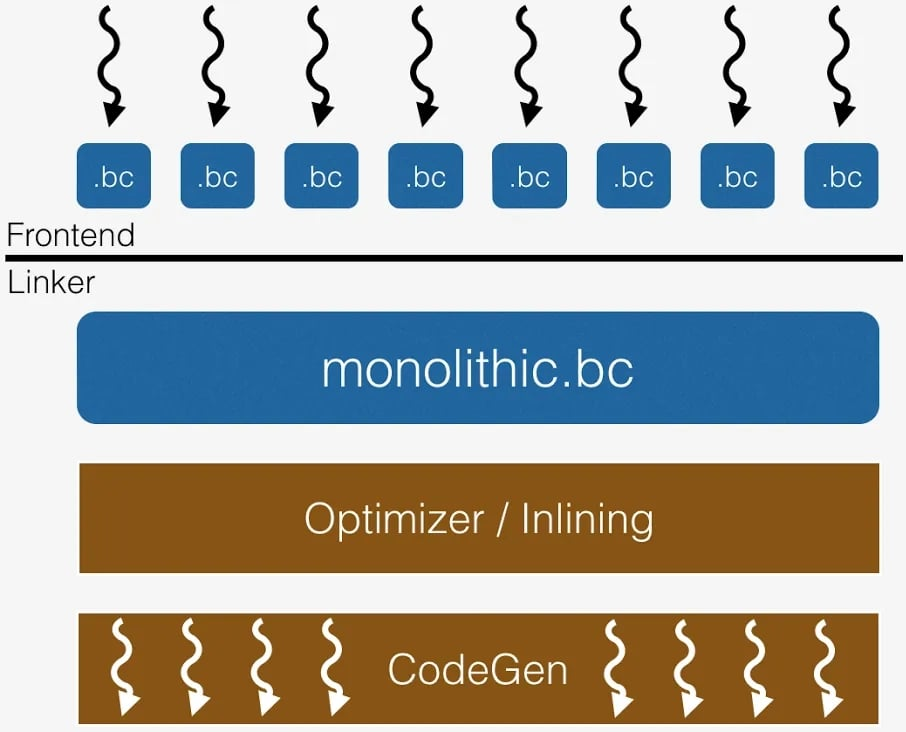
\includegraphics[width=0.8\textwidth]{LTO_normal.png}
  \caption{Стандардни процес оптимизације током линковања}
  \label{fig:grafikon}
\end{figure}

Стандардни приступ има неколико мана.
Први проблем је то што губимо предности паралелног компајлирања, која постоји 
када није активна оптимизација целовитог програма.
Као што видимо на слици 4.1 постоји паралелно превођење изворних фајлова у 
битк\^{o}д фајлове али због спајања свих фајлова у један велики битк\^{o}д фајл,
ту предност касније губимо зато што све оптимизације над тим фајлом морају 
да се раде без могућности парелелизације.
Због тога компајлирање траје много дуже него без оптимизације целовитог програма.
Такође, за сваку промену у било ком изворном фајлу, ми поново морамо испочетка
вршити све оптимизације на обједињеном фајлу, што поново изузетно утиче не време
превођења.
Још један велики проблем овог приступа је меморијско заузеће.
Због тога што сада у меморији морају да се налазе све међурепрезентације, спојене
у једну, често је немогуће извршити оптимизацију целовитог програма, поготово на 
машинама које немају велику радну меморију.
Приступ за решавање ових проблема је  ThinLTO[20].
\par ThinLTO је нови приступ који омогућава сличне перфомансе при превођењу
као када није укључена оптимизација целовитог програма, док задржава већину
оптимизација и самим тим перфоманси извршног фајла као регуларна оптимизација
целовитог програма.
При ThinLTO оптимизацији уместо учитавања битк\^{o}д фајлова и спајања у један,
већ за сваку јединицу транслације и сваку функцију или глобал у њој, чува кратак
резиме за анализу у кораку линковања. 
Кључна оптимизација коју ThinLTO омогућава је убацивање само оних функција које
су потребне конкретном битк\^{o}д фајлу и које ће бити инлајноване у том  битк\^{o}д фајлу.
И тај поступак радимо за сваки  битк\^{o}д фајл, што значи да нема спајања, већ се и
даље поступак  извршава паралелно.
ThinLTO процес оптимизације целовитог програма је подељен на 3 фазе:
\begin{enumerate}
\item Превођење - генеришу се међурепрезензације као и случају стандардног процеса
	оптимизације целовитог програма, са тим што сада имамо и резиме уз сваку
	међурепрезентацију
\item Линковање - линкер комбинује резимее из прошлог корака и врши анализу
\item Бекенд - Паралелна оптимизација и генерисање к\^{o}да
\end{enumerate}
 
\begin{figure}[!ht]
  \centering
  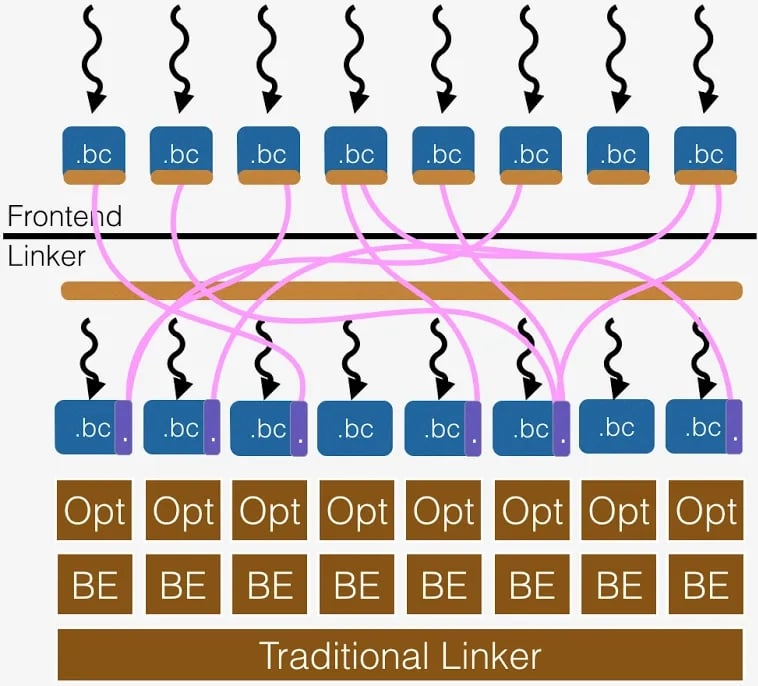
\includegraphics[width=0.8\textwidth]{LTO_thin.png}
  \caption{ThinLTO процес оптимизације}
  \label{fig:grafikon}
\end{figure}

Кључни део ThinLTO оптимизације се дешава у првој фази, а то су креирања резимеа.
Свака глобална променљива и функција се налазе у резимеу, за ту јединицу транслације.
Резиме садржи по једно поље за сваки симбол и у том пољу
се налазе подаци који описују тај симбол.
На пример, за функцију, у пољу унутар резимеа може да стоји њена видљивост, 
број инструкција које функција садржи, информације за профајлирање уколико су потребне
и слично.
Додатно, свака референца према другом симболу(позив друге функције, узимање адресе,
приступање глобалу) се записује у резиме и тако се гради граф контроле тока(eng. call graph).
Ове информације омогућавају креирање комплетног графа током фазе линковања.
ThinLTO је једноставно активирати, само је потребно додати  -flto=thin у командној линији
приликом компајлирања.

//todo bencmarci


% ------------------------------------------------------------------------------
\chapter{Закључак}
% ------------------------------------------------------------------------------



% ==============================================================================
% Završni deo teze i prilozi
\backmatter
% ==============================================================================
\chapter{Литература}
[1] LLVM Compiler Infrastructure -- https://llvm.org/docs/index.html \\

[2] LLVM Language Reference Manual -- https://llvm.org/docs/LangRef.html \\

[3] SSA Form -- https://en.wikipedia.org/wiki/Static{\_}single{\_}assignment{\_}form \\
 
[4] RISC -- https://en.wikipedia.org/wiki/Reduced{\_}instruction{\_}set{\_}computer \\

[5] Abstract Syntax tree -- https://en.wikipedia.org/wiki/Abstract{\_}syntax{\_}tree \\

[6] Optimizer -- https://llvm.org/docs/CommandGuide/opt.html \\

[7] LLVM Code Generator -- https://llvm.org/docs/CodeGenerator.html \\

[8] Just In Time Compilation  -- https://en.wikipedia.org/wiki/Just-in-time{\_}compilation \\

[9] Clang Static Code Analyzer  -- https://clang-analyzer.llvm.org/ \\ 

[10] Link Time Optimization -- https://llvm.org/docs/LinkTimeOptimization.html \\

[11] libLTO -- https://llvm.org/docs/LinkTimeOptimization.html{\#}liblto \\

[12] Gold linker -- https://llvm.org/docs/GoldPlugin.html \\

[13] llvm-link -- https://llvm.org/docs/CommandGuide/llvm-link.html \\

[14] Function inlining -- https://www.cs.cornell.edu/courses/cs6120/2019fa/blog/llvm-function-inlining/ \\

[15] Indirect branch instructions -- https://en.wikipedia.org/wiki/Indirect{\_}branch \\

[16] Dead code elimination -- https://en.wikipedia.org/wiki/Dead{\_}code{\_}elimination \\

[17] Devirtualization -- https://blog.llvm.org/2017/03/devirtualization-in-llvm-and-clang.html \\

[18] Internal linkage -- https://www.learncpp.com/cpp-tutorial/internal-linkage/ \\

[19] Unnamed namespace -- https://www.ibm.com/docs/en/i/7.3?topic=only-unnamed-namespaces-c \\

[20] ThinLTO -- https://clang.llvm.org/docs/ThinLTO.html
\end{document} 
